\documentclass[conference]{IEEEtran}
\IEEEoverridecommandlockouts
\usepackage{cite}
\usepackage{amsmath,amssymb,amsfonts}
\usepackage{algorithm}
\usepackage{algpseudocode}
\usepackage{graphicx}
\usepackage{textcomp}
\usepackage{xcolor}
\usepackage{booktabs}
\usepackage{multirow}
\usepackage{threeparttable}
\usepackage{pgfplots}
\usepackage{tikz}
\usetikzlibrary{arrows.meta,positioning,shapes.geometric,calc,fit,backgrounds}
\pgfplotsset{compat=1.17}
\usepackage[hidelinks]{hyperref}

\newcommand{\acc}[1]{\textrm{A@}#1}
\def\BibTeX{{\rm B\kern-.05em{\sc i\kern-.025em b}\kern-.08em T\kern-.1667em\lower.7ex\hbox{E}\kern-.125emX}}

\begin{document}

\title{Evidence-Weighted Hybrid Detection, Learned Topology\\ and Calibrated Cascade Modelling for Instrumentation-Free\\ Root-Cause Analysis in Microservice Systems}

\author{\IEEEauthorblockN{Anish C, Dhanush K Murthy, K Bharath Parmar, Royson Salis}
\IEEEauthorblockA{\textit{Department of Artificial Intelligence and Machine Learning}\\
\textit{Mangalore Institute of Technology and Engineering}\\
Mangalore, India}}

\maketitle

\begin{abstract}
When a microservice fails, the failure does not stay where it starts: a slow datastore drags down the services that query
it, their callers time out, retry layers amplify the load, and within a minute an operator faces dozens of simultaneous
alarms in which the originating fault is indistinguishable, by severity alone, from the services merely suffering its
effects. Recent diagnosis methods localise the fault with graph neural networks over fused metrics, traces and logs; they
are effective but need labelled failures, GPU inference and produce an output the on-call engineer cannot audit. We take
the opposite position and keep the whole pipeline unsupervised, single-core, auditable and free of application
instrumentation, discovering the dependency graph from outside the application over SSH. On that base we contribute a
hybrid detector that combines per-service online Isolation Forests with a robust statistical rule layer under an
operator-chosen false-alarm budget; a root-cause ranker that separates a service's own deviation from the part its
neighbours explain and runs a personalised-PageRank walk over the dependency graph; a dependency graph whose call
directions are \emph{learned from telemetry} rather than guessed from service names; a calibrated cascade model that
predicts which healthy services an incident will reach; and online change-point detection that shortens detection latency.
We evaluate on 217 minutes of real telemetry from two containerised benchmark systems with 62 faults injected blind to the
detector, and on a held-out synthetic benchmark of 178 faults across 16 topologies. The hybrid engine catches and names
the correct root cause in 74\% of real incidents against 53\% for a calibrated severity baseline, while spending less
fault-free time in alarm (7\% against 11\%). Learned directions match a perfect-topology ceiling for ranking (71\% vs
73\%) and, unlike the name rule, do not collapse when names are uninformative (28/31 vs 0/31 correct). Change-point alarms
roughly halve the median detection delay on the real benches (10.5\,s to 4.9\,s). We report an ablation that isolates each
mechanism, a controlled study of when the graph terms become decisive, and two honest negative results. The pipeline
needs no training, no labels and no GPU, and costs under 7\,ms per five-second window on a thirteen-service graph.
\end{abstract}

\begin{IEEEkeywords}
AIOps, anomaly detection, calibration, cascading failures, causal discovery, change-point detection, dependency graph,
isolation forest, microservices, root cause analysis.
\end{IEEEkeywords}

\section{Introduction}
Microservice architectures decompose an application into many small services that communicate over the network
\cite{dragoni2017microservices}. The style buys independent deployment and horizontal scaling, and it introduces a failure
mode that monolithic systems do not have: a fault does not stay where it starts. When a database slows, the service
querying it slows while waiting; the services calling that service time out; a retry layer amplifies the load; and within a
minute a dozen services are alarming at once. Practitioners call the result an alert storm, and its cost is not the alerts
themselves but the time an engineer spends deciding which one to act on \cite{beyer2016sre}.

Two properties of this phenomenon make it tractable. First, failures propagate along the call graph, from a callee to the
callers that wait on it, and not arbitrarily. Second, propagation is probabilistic rather than certain: a caller protected
by a timeout, a cache or a circuit breaker may survive a failing dependency while an unprotected one will not. A system
that knows the call graph, and knows how likely propagation is along each edge, can therefore answer two questions that a
ranked alert list cannot: which service is most likely to be the origin, and which services not yet affected are about to
be pulled in.

Recent work answers the first question with increasingly heavy machinery. Multimodal methods fuse metrics, traces and logs
into learned representations over temporal knowledge graphs and localise failures with relation-aware graph convolution or
graph autoencoders \cite{zhang2023diagfusion,sun2024deephunt,lee2023eadro}. They are effective, and they carry three costs
that matter in practice: they need labelled or curated failure data that most organisations do not have; they need GPU
inference, which pushes them out of the real-time path; and they produce an output, a cluster identifier or an embedding
ranking, that the engineer who must act on it cannot check against the underlying measurement.

We argue that the information which actually discriminates a cause from a victim is \emph{structural}, and that it is
available cheaply. This paper therefore keeps the detector simple, explicit and calibrated, and spends the modelling effort
on the graph and on the way evidence flows across it. Two design decisions are central. First, the dependency graph is not
a fixed adjacency matrix but a body of evidence: an edge declared in a deployment file but never observed carrying traffic
is weaker evidence of a causal pathway than an edge seen carrying a hundred connections a minute, and the difference is
quantified and propagated into scoring, ranking and cascade prediction rather than merely displayed. Second, where the live
engine still relies on a heuristic, namely recovering call directions from service names, we show the heuristic can be
replaced by a quantity learned from the telemetry itself, with no loss on named systems and a large gain on systems whose
names carry no information.

\subsection{Contributions}
\begin{enumerate}
\item \textbf{An instrumentation-free, evidence-weighted dependency graph.} Every edge carries a confidence
$w_{u\to v}\in[0,1]$ derived from whether it is declared, whether it was observed carrying traffic, how busy it is, and how
its direction was resolved. The graph is discovered over SSH with no code changes, and the confidence is consumed by the
models (Section~\ref{sec:graph}).
\item \textbf{A hybrid detector with an operational contract.} Per-service online Isolation Forests, split into an
intrinsic (resource) group and a symptom group, run alongside a robust statistical rule layer; either can raise the alarm.
The project-level threshold is chosen against an explicit false-alarm budget, and we show that measuring alarm \emph{time}
rather than alarm \emph{episodes} is necessary to make that contract honest (Section~\ref{sec:detect}).
\item \textbf{A deviation decomposition and a walk-based ranker.} Each service's abnormality is split into the part its
neighbours explain and the part they do not, and a personalised-PageRank walk over the evidence-weighted graph collects
root-cause mass at the service whose trouble nothing downstream accounts for (Section~\ref{sec:rca}).
\item \textbf{Learned call directions.} We replace the name-based direction heuristic with a direction learned online from
lagged implication, cross-correlation and traffic ratio. It matches a perfect-topology ceiling and is robust to
uninformative names (Section~\ref{sec:learned}).
\item \textbf{A calibrated cascade model and early warning.} A per-edge propagation probability, a Beta--Binomial
posterior whose prior is the edge's evidence, drives an independent-cascade prediction of which services will be reached;
online change-point detection shortens detection latency and gives early warning on gradual faults
(Section~\ref{sec:cascade}).
\item \textbf{An honest, reproducible evaluation.} A mapper-blind fault injector produces ground truth independent of the
detector; a synthetic generator extends the sample to sixteen topologies; and we report an ablation, a controlled
amplifying-regime study, two negative results and a measurement bug we found and corrected (Sections~\ref{sec:setup}
and~\ref{sec:results}).
\end{enumerate}

\section{Related Work}
\textbf{Unsupervised anomaly detection.} Isolation Forest \cite{liu2008isolation,liu2012isolation} isolates an outlier with
few random axis-parallel cuts and needs no density estimate, which suits per-service streams with mixed, skewed metrics.
Distance and density baselines \cite{ramaswamy2000efficient,breunig2000lof}, the histogram score HBOS
\cite{goldstein2012hbos} and the multivariate control chart of Hotelling \cite{hotelling1931,mahalanobis1936} with
shrinkage covariance \cite{ledoit2004} are natural alternatives; we compare all of them. Robust location and scale from the
median and MAD \cite{hampel1974,rousseeuw1993} underpin our rule layer. Surveys of streaming and deep anomaly detection
\cite{gama2014survey,chandola2009survey} and critiques of evaluation practice \cite{wu2021flawed,kim2022rigorous} motivate
our event-level, budget-based protocol over point-wise F1 with point adjustment \cite{tatbul2018precision}.

\textbf{Root-cause localisation.} MonitorRank \cite{kim2013monitorrank} introduced the personalised random walk over the
call graph that we adopt; MicroRCA \cite{wu2020microrca}, CloudRanger \cite{wang2018cloudranger}, Microscope
\cite{lin2018microscope}, AutoMAP \cite{ma2020automap} and MicroRank \cite{yu2021microrank} extend it with anomaly-weighted
transitions and trace spectra. Causal approaches recover structure with the PC algorithm or hierarchical causal discovery
\cite{ikram2022rcd,li2022circa,xin2023causalrca}, and learned methods localise with graph autoencoders and multi-source
fusion \cite{sun2024deephunt,zhang2023diagfusion,lee2023eadro,wang2021groot}. These need traces or training; our ranker
needs neither, and our learned-direction module borrows the spirit of causal discovery while staying a cheap online
statistic.

\textbf{Cascade and change.} Influence spread under the independent-cascade model \cite{kempe2003influence} is the basis of
our propagation prediction, with edge probabilities estimated online as Beta--Binomial posteriors. Detection latency is
attacked with classical change-point detection: the CUSUM chart \cite{page1954cusum} and Bayesian online change-point
detection \cite{adams2007bocpd}. Personalised PageRank \cite{page1999pagerank} and reciprocal-rank fusion
\cite{cormack2009rrf} inform the ranking; Granger causality \cite{granger1969} and transfer entropy \cite{schreiber2000te}
inform the direction study. Random forests and CART \cite{breiman2001rf,breiman1984cart} back the fault-type classifier.
Chaos-engineering practice \cite{basiri2016chaos} and open benchmark applications \cite{gan2019deathstar,zhou2018trainticket}
frame our fault-injection methodology.

\section{Instrumentation-Free Collection and the Evidence-Weighted Graph}
\label{sec:graph}

\begin{figure}[t]
\centering
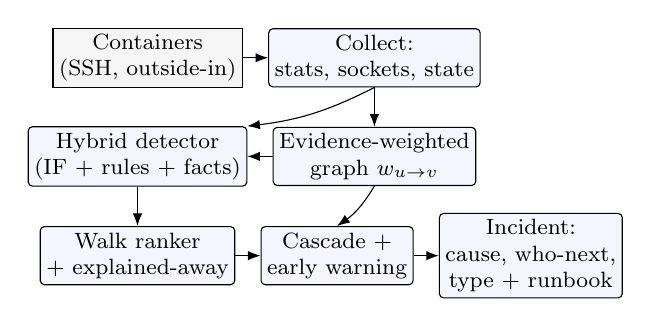
\begin{tikzpicture}[font=\footnotesize,node distance=3.2mm,
  box/.style={draw,rounded corners=1.5pt,align=center,inner sep=2.2pt,minimum height=6.5mm,fill=blue!4},
  dat/.style={draw,align=center,inner sep=2.2pt,minimum height=6.5mm,fill=gray!8},
  ar/.style={-{Latex[length=1.6mm]}}]
\node[dat] (host) {Containers\\(SSH, outside-in)};
\node[box,right=of host] (col) {Collect:\\stats, sockets, state};
\node[box,below=5mm of col] (graph) {Evidence-weighted\\graph $w_{u\to v}$};
\node[box,left=of graph] (det) {Hybrid detector\\(IF + rules + facts)};
\node[box,below=5mm of det] (rca) {Walk ranker\\+ explained-away};
\node[box,right=of rca] (cas) {Cascade +\\early warning};
\node[box,right=of cas] (out) {Incident:\\cause, who-next,\\type + runbook};
\draw[ar] (host)--(col); \draw[ar] (col)--(graph); \draw[ar] (col.south) to[bend left=10] (det.north east);
\draw[ar] (graph)--(det); \draw[ar] (det)--(rca); \draw[ar] (graph.south) to[bend left=12] (cas.north);
\draw[ar] (rca)--(cas); \draw[ar] (cas)--(out);
\end{tikzpicture}
\caption{The pipeline. Everything is computed outside the application from container telemetry; the evidence-weighted
graph feeds detection, ranking and cascade prediction.}
\label{fig:pipeline}
\end{figure}

\textbf{Collection.} Every five seconds the collector lists all containers (including stopped ones), reads CPU, memory,
network byte rates and restart counts from the container runtime, and reads the established TCP sockets inside each
container from \texttt{/proc/net/tcp}. Missing readings are recorded as \emph{unknown}, never as zero, so that silence from
a stopped container is distinguishable from a container idling at zero. A connection's direction is oriented from listening
versus ephemeral ports, and the evidence for that orientation is recorded rather than discarded.

\textbf{Edge confidence.} An edge $A\to B$ means ``$A$ calls $B$'', so failure travels against the arrow. The confidence of
an edge is the strongest evidence behind it: $1.0$ for a call seen in request logs or oriented by a listening port, $0.85$
when the direction comes only from the ephemeral-port range, $0.70$ when observed without direction evidence, $0.50$ when
the direction is unresolved, and $0.40$ when the edge is declared in the deployment configuration but never seen carrying
traffic. The \emph{dependency share} $d(e)$ of an edge out of a caller is its baseline traffic normalised over the caller's
other edges, computed from a slow baseline of socket activity rather than the instantaneous rate, because a link goes quiet
exactly when its callee dies. The scalar weight is $w(e)=\mathrm{clip}(c(e)\cdot d(e)\cdot \phi,\,0,\,1)$, where $\phi$
discounts fire-and-forget telemetry edges. This weight is the single structural quantity consumed by the ranker and the
cascade model.

\section{Hybrid Detection}
\label{sec:detect}
A service is judged against its own recent past, never against a global threshold, because services differ by orders of
magnitude in every metric.

\textbf{Per-service Isolation Forests.} Each reading becomes eight features: CPU, memory, throttling, network in and out,
request rate, error share and p95 latency, with positive quantities on a log scale. The features are split into two groups,
each with its own forest of 100 trees trained on a sliding window of the last 120 readings judged normal:
\emph{own} (CPU, memory, throttling), which a dependency cannot cause, and \emph{symptom} (traffic, errors, latency,
network), which can be inherited. A reading is scored by the forest built \emph{before} it arrived. The raw score
$s(x)=2^{-\mathbb{E}[h(x)]/c(\psi)}$ is turned into a level
\begin{equation}
\mathrm{level}(x)=\frac{s(x)-\tilde s}{\ell-\tilde s},\qquad
\ell=\tilde s + \kappa\cdot 1.4826\cdot \mathrm{MAD}(s_{\mathrm{train}}),
\end{equation}
where $\tilde s$ is the median training score and the robust line $\ell$ ($\kappa=3$) does not drift with the random trees.
Four refinements were each found by testing and each validated in the ablation of Section~\ref{sec:results}:
\emph{(i) training jitter} at each feature's floor, so a feature that never moved in the window can still register a later
jump; \emph{(ii) a range guard} that counts how many floors a reading sits beyond the training range, because a forest
scores an out-of-range value no higher than its most extreme training point; \emph{(iii) one-sided features}, so that less
CPU, memory, throttling, error or latency than usual is never a fault of the service itself, which removes a persistent
false alarm after every restart; and \emph{(iv) two-speed drift}, where a small steady shift is accepted as the new normal
within two minutes while a large shift is quarantined for thirty, so a genuine fault never becomes the baseline.

\textbf{Rule layer and facts.} In parallel, a robust one-sided z-score per metric (median and MAD, with the bad direction
only) gives a rule score normalised so that $1$ is its three-sigma line. Container facts, a service that is exited, paused,
restarting or network-detached, are treated as evidence rather than degree. Two facts that the plain container state misses
were added after inspecting the real runs: a \texttt{docker stop} exits with code zero, which looks like a finished job, so
a service that had been running and then exits is treated as stopped; and a crash loop looks healthy between kills, so two
outages within three minutes mark it.

\textbf{The hybrid and its contract.} The project alarms when some service reaches twice its own line for two consecutive
windows, or when the rule layer is well past its line on its own, or on any hard fact. The threshold is chosen to respect a
false-alarm budget of $B$ episodes per fault-free hour, which is a quantity an operator can choose, unlike a sigma value.
We stress one methodological point. An engine can satisfy a per-hour episode budget while alarming almost continuously,
because one unbroken alarm is a single episode. We therefore report \emph{alarm time}, the fraction of fault-free time in
alarm, alongside the episode rate; it exposed that an earlier version of our own detector, which looked excellent on
episodes, was in alarm 86\% of the time. Refinements (iii) and (iv) bring that to 5\%.

\section{Root-Cause Ranking}
\label{sec:rca}
The question is which of the unwell services is the source. A caller's errors are usually inherited, so the engine separates
own evidence from symptoms and lets a broken dependency explain away its callers.

\textbf{Explained-away.} For service $s$ with own level $o(s)$ and symptom level $\sigma(s)$, and callees $C(s)$,
\begin{align}
x(s)&=\gamma\max_{c\in C(s)} a(c),\nonumber\\
\mathrm{raw}(s)&=\max\!\big(o(s),\,\max(0,\sigma(s)-x(s))\big),
\end{align}
where $a(\cdot)$ is the anomaly in $[0,1]$ and $\gamma$ scales the discount by edge confidence. A service whose symptoms are
fully explained by a sick callee drops out; a service abnormal in its own resources does not.

\textbf{The walk.} We rank with a personalised-PageRank walk in the MonitorRank form \cite{kim2013monitorrank}. A walker on
the evidence-weighted graph steps forward to a callee with weight $w(u\to v)\,a(v)$, back to a caller with weight
$\rho\,a(u)$, and stays with weight $\max(0, a(u)-\max_{c}a(c), o(u))$, and restarts on the anomalous set with probability
$\alpha$. The stationary share is the root-cause score; hard facts are ranked first. The stay term is what makes the source,
whose trouble nothing downstream explains, collect the most mass.

\section{Learned Call Directions}
\label{sec:learned}
A walk needs directed edges, but the collector sees most pairs from both ends, so direction must be recovered. The live
engine infers it from service names (a gateway calls a database), which fails on systems whose names carry no role. We learn
the direction of each observed pair online from three signals computed on the services' own histories: a lagged implication
statistic (how often one service's anomaly onset precedes the other's among connected, concurrently anomalous services),
the lag of peak cross-correlation of the error, latency and request-rate series, and the traffic ratio, since a callee's
request rate tracks its caller's. The signals vote, and the pair is oriented toward the leader. The rule is purely a
statistic over the past; it adds no training and no labels. Section~\ref{sec:results} shows it matches a perfect-topology
ceiling for ranking and, unlike the name rule, is unaffected when names are stripped.

\section{Cascade Prediction and Early Warning}
\label{sec:cascade}
\textbf{Who is hit next.} Each call edge carries a propagation probability estimated online. Every time a service turns
abnormal, each healthy caller is a trial: did it turn abnormal within one minute? The success rate is a Beta--Binomial
posterior whose prior is the edge's evidence confidence and weight $\pi_0$ of strength $m$,
\begin{equation}
p(c\!\leftarrow\!x)=\frac{\text{successes}+m\,\pi_0}{\text{trials}+m},
\end{equation}
so a rarely exercised edge starts at its evidence prior and moves with observation. Risk then flows up the call graph from
the current suspect by noisy-OR, the independent-cascade model \cite{kempe2003influence},
\begin{equation}
P(c)=1-\!\!\prod_{x\in C(c)}\!\!\big(1-P(x)\,p(c\!\leftarrow\!x)\big),\quad P(\text{suspect})=1,
\end{equation}
and services above a risk cut are shown as likely-next.

\textbf{Early warning.} For each rising-only feature a least-squares trend is fitted over the last two minutes and projected
two minutes ahead through the range guard; a service not yet over its line whose trend will cross it is flagged. This fires
on gradual faults, memory leaks and throttling, where there is a slope to extrapolate.

\textbf{Earlier detection.} In parallel, online change-point detectors (Page--Hinkley, CUSUM \cite{page1954cusum} and
Bayesian online change-point detection \cite{adams2007bocpd}) run on the raw metrics and can raise the alarm before the
forest line is crossed; their onset times also feed the direction study and a temporal-precedence ranker.

\section{Fault Diagnosis}
\label{sec:diagnose}
Once an incident is raised and a suspect named, a 35-feature vector is read from the suspect's telemetry up to the alarm and
a short window after it: container-state history, exit code, restart count and number of separate outages, memory slope,
CPU and throttling change, latency and error ratios against a pre-fault baseline, network drop, and how many callers are
anomalous. A hand-written random forest \cite{breiman2001rf} names the fault class (crash, stop, pause, crash-loop, flap,
memory, brownout, latency, partition) and a per-class runbook of two to four concrete checks is attached. The classifier is
a convenience layer on top of the ranker, not a change to detection.

\section{Experimental Setup}
\label{sec:setup}
\textbf{Systems.} Two containerised benchmark applications instrumented in the OpenTelemetry style: \emph{ShopFlow}, a
13-service retail checkout system (HTTP fan-out, two Postgres instances, two Redis caches, a NATS consumer), and
\emph{LedgerLine}, a 12-service retail-banking transfer system (a saga orchestrator, a double-entry ledger, a third-party
FX provider behind a breaker, a batch worker). Together they run for 217 minutes under organic, open-loop traffic.

\textbf{Mapper-blind fault injection.} Faults arrive as a non-homogeneous Poisson process whose rate follows the daily load
curve; each fault draws a class, a target weighted by role, a heavy-tailed duration and a severity, and with some
probability spawns a follower in the target's one-hop neighbourhood, so incidents overlap. Faults are physical
(\texttt{SIGKILL}, pause, cgroup CPU and memory limits, network detach); nothing is labelled, logged or signalled inside
the system under test, so the detector is blind to the plan. The injector writes a private ledger with, per fault, the true
root cause and the set of services structurally able to be affected; the ledger is read only after the run, to score. The
two runs contain 62 faults across seven classes.

\textbf{Synthetic benchmark.} To enlarge the sample we built a generator that writes runs in the identical recorded format,
reproducing the two topologies with their measured per-service baselines plus random topologies, traffic waves and bursts,
nine fault classes that propagate up and down the graph, overlapping faults and unlabelled noise (noisy neighbours,
deploys, missing readings). Settings are chosen on a 16-campaign tuning split and reported once on a disjoint 16-campaign,
178-fault held-out split.

\textbf{Metrics.} We use event-level scoring, not point-wise. A fault is \emph{detected} when an alarm during it (or within
a grace window) places a truly involved service in the top three; it is \emph{caught and named} when, in addition, the
faulted service is ranked first (\acc{1}); false alarms are alarm episodes outside every fault window, per fault-free hour;
alarm time is the fraction of fault-free time in alarm. The cascade model is scored by AUROC-free precision, recall and F1
of the who-next set, and by calibration. All decisions are causal, using only the past.

\textbf{Protocol honesty.} During this study we found that each recorded run contains two fault campaigns that both number
their faults from one, and the ledger reader kept only the second campaign, hiding 14 of 31 faults per bench for every
engine and counting their outages as false alarms. We fixed the reader, added a regression test, and all numbers below use
the full 62 faults.

\section{Results}
\label{sec:results}
\subsection{Detection and root cause}
Table~\ref{tab:main} compares the rule layer, the ML engine and the hybrid in one harness on the real benches, and on the
held-out synthetic split. On the real benches the hybrid names the right service first in 74\% of incidents against 65\% for
the rules alone, detects as many faults, and spends less fault-free time in alarm. The ML engine alone is the most precise
ranker but misses a few faults that the rule layer catches; the hybrid recovers them. Figure~\ref{fig:bars} shows the same
on \acc{1}.

\begin{table}[t]
\centering
\caption{Detection and root cause, one harness. Real: 62 faults, 2 systems. Synthetic: 178 held-out faults, 16 topologies.}
\label{tab:main}
\footnotesize
\begin{tabular}{llcccc}
\toprule
Set & Engine & Det. & \acc{1}$^\dagger$ & C+N & Alarm \\
 & & (\%) & (\%) & (\%) & time \\
\midrule
\multirow{3}{*}{Real}
 & Rules      & 90 & 71 & 65 & 9\% \\
 & ML         & 87 & 83 & 73 & 5\% \\
 & \textbf{Hybrid} & \textbf{90} & \textbf{82} & \textbf{74} & 7\% \\
\midrule
\multirow{3}{*}{Synthetic}
 & Rules      & 89 & 78 & 70 & 2\% \\
 & ML         & 89 & 78 & 70 & 1\% \\
 & \textbf{Hybrid} & \textbf{92} & \textbf{79} & \textbf{72} & 2\% \\
\bottomrule
\end{tabular}
\\[2pt]
{\scriptsize $^\dagger$\acc{1} among detected faults. C+N (caught and named) = detected and ranked first, over all faults.}
\end{table}

\begin{figure}[t]
\centering
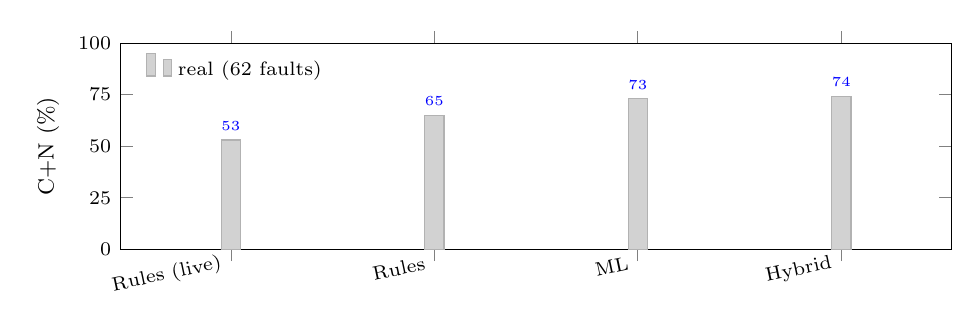
\begin{tikzpicture}
\begin{axis}[width=\columnwidth,height=4.2cm,ybar,bar width=7pt,ymin=0,ymax=100,
  ylabel={C+N (\%)},ylabel style={font=\footnotesize},
  symbolic x coords={Rules (live),Rules,ML,Hybrid},xtick=data,
  x tick label style={font=\scriptsize,rotate=12,anchor=east},
  ytick={0,25,50,75,100},tick label style={font=\scriptsize},
  legend style={font=\scriptsize,at={(0.02,0.98)},anchor=north west,draw=none},
  nodes near coords,every node near coord/.append style={font=\tiny},
  enlarge x limits=0.18]
\addplot+[fill=gray!35,draw=gray!60] coordinates {(Rules (live),53)(Rules,65)(ML,73)(Hybrid,74)};
\addlegendentry{real (62 faults)}
\end{axis}
\end{tikzpicture}
\caption{Root cause caught and named first on the real benches. ``Rules (live)'' is the detector as shipped before this
study's refinements; the others are in the common harness.}
\label{fig:bars}
\end{figure}

\textbf{Cross-system generalisation.} Choosing the ML settings on one bench and testing untouched on the other, the ML
ranker reaches \acc{1} of 85\% on ShopFlow and 78\% on LedgerLine, against 64\% and 56\% for the live rules, confirming the
ranking advantage transfers across architectures.

\textbf{By fault class.} On the real benches the hybrid names every crash (16/16), stop (16/16), pause (4/4) and flap (2/2),
most memory leaks (4/6) and crash loops (3/4), and almost no brownouts (1/14). Brownouts are the open problem: many strike
near-idle services where CPU throttling barely shows in the telemetry.

\subsection{Ablation}
Table~\ref{tab:abl} removes one mechanism at a time on the real benches (three seeds). The single most important component
for root cause is the \texttt{docker stop} fact: without it, caught-and-named falls from 72\% to 53\% and detection from
88\% to 82\%, because every stopped service goes unnamed. One-sided features and the alarm-at-twice-the-line rule are what
keep alarm time at 5\%: removing the former raises it to 30\%, removing the latter to 22\% and the false-alarm rate to
11.3/h. The random walk and the crash-loop fact each contribute a few points of \acc{1}.

\begin{table}[t]
\centering
\caption{Ablation on the real benches (mean over 3 seeds). Each row removes one mechanism from the full engine.}
\label{tab:abl}
\footnotesize
\begin{tabular}{lcccc}
\toprule
Configuration & Det. & \acc{1} & C+N & Alarm \\
 & (\%) & (\%) & (\%) & time \\
\midrule
Full engine (default)      & 88 & 81 & 72 & 5\% \\
\;$-$ \texttt{docker stop} fact   & 82 & 65 & 53 & 5\% \\
\;$-$ one-sided features          & 92 & 76 & 70 & 30\% \\
\;$-$ alarm at $2\times$ line     & 94 & 78 & 74 & 22\% \\
\;$-$ crash-loop fact             & 88 & 78 & 69 & 5\% \\
\;$-$ range guard                 & 83 & 82 & 68 & 0\% \\
\;$-$ random walk                 & 88 & 79 & 69 & 5\% \\
\bottomrule
\end{tabular}
\end{table}

\textbf{Detector choice.} Swapping the Isolation Forest for k-nearest-neighbours, Mahalanobis or HBOS, each under the same
window, line and range guard, gives comparable or slightly higher \acc{1} (77\%, 74\%, 71\%) but 16 to 23 false alarms per
hour and 20 to 41\% alarm time, against 2.1/h and 5\% for the forest. The forest is kept for its quietness, not its ranking.

\subsection{Learned directions}
Table~\ref{tab:dir} reports direction accuracy on the observed pairs that are real calls. With names available the learned
rule is already better than the name heuristic (28 vs 21 of 31 correct on the real benches, and it leaves none unresolved).
When service names are stripped, the name heuristic collapses to zero while the learned rule is unchanged. Fed to the walk,
learned directions reach caught-and-named 71\% on the real benches against a 73\% ceiling from the true graph and 68\% with
no directions at all, and against 69\% for the name rule once names are hidden. Directions are worth about six points of
root cause, and the learned ones recover almost all of it without reading names.

\begin{table}[t]
\centering
\caption{Call-direction accuracy on observed pairs that are true calls (correct / wrong / unresolved).}
\label{tab:dir}
\footnotesize
\begin{tabular}{llcc}
\toprule
Set & Method & Names shown & Names hidden \\
\midrule
\multirow{2}{*}{Real (31)}
 & Name rule & 21 / 0 / 10 & \phantom{0}0 / 0 / 31 \\
 & Learned   & 28 / 3 / \phantom{0}0 & 28 / 3 / \phantom{0}0 \\
\midrule
\multirow{2}{*}{Synthetic (204)}
 & Name rule & 172 / 0 / 32 & \phantom{0}95 / 0 / 109 \\
 & Learned   & 197 / 6 / \phantom{0}1 & 197 / 6 / \phantom{00}1 \\
\bottomrule
\end{tabular}
\end{table}

\subsection{Cascade, early warning and change-point}
The cascade model's who-next prediction has F1 comparable to predicting the entire upstream set, but at higher precision
(synthetic F1 0.43 at precision 0.40 against 0.45 at precision 0.32; real 0.17 against 0.14). Predicting the next affected
service accurately is hard for every method, and we do not overclaim it. The trend forecaster gives early warning before the
alarm on gradual faults: 16 of 178 synthetic faults, median lead 30\,s, concentrated on memory leaks (7 of 18); it almost
never fires on the abrupt real faults (1 of 62). Change-point alarms are the clear latency win: on the real benches they cut
the median detection delay from 10.5\,s to 4.9\,s and lift detection from 90\% to 95\%, for about 1.5 extra false alarms per
hour (Fig.~\ref{fig:delay}).

\begin{figure}[t]
\centering
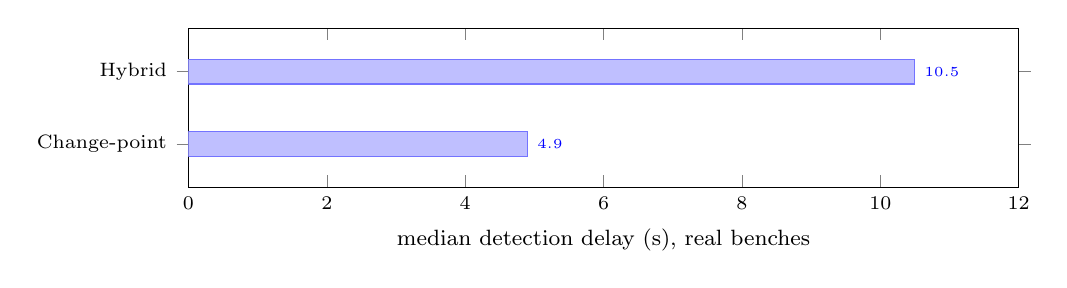
\begin{tikzpicture}
\begin{axis}[width=\columnwidth,height=3.6cm,xbar,bar width=9pt,xmin=0,xmax=12,
  xlabel={median detection delay (s), real benches},xlabel style={font=\footnotesize},
  symbolic y coords={Change-point,Hybrid},ytick=data,
  tick label style={font=\scriptsize},
  nodes near coords,every node near coord/.append style={font=\tiny},
  enlarge y limits=0.6]
\addplot+[fill=blue!25,draw=blue!55] coordinates {(10.5,Hybrid)(4.9,Change-point)};
\end{axis}
\end{tikzpicture}
\caption{Online change-point alarms roughly halve the median detection delay on the real benches.}
\label{fig:delay}
\end{figure}

\subsection{Fault diagnosis}
Thirty seconds after the alarm, the random-forest classifier reaches 77\% accuracy and 0.73 macro-F1 on the held-out
synthetic split, and 99\% when given the true service, which shows the bottleneck is naming the suspect, not the class: when
the engine names the right service, the class is almost always right. On the real benches the hand-written decision list
transfers best (59\% on the engine's suspect, 84\% on the true service), because the learned models pick up
synthetic-specific patterns; real flaps are pause cycles and real brownouts on idle services show no throttling.

\subsection{Cost}
The whole pipeline is unsupervised, needs no GPU and runs on a single core. Detection, ranking and cascade for a
thirteen-service graph cost under 7\,ms per five-second window end to end, roughly 0.5\,ms per service, with the per-service
forests linear in the number of services and the walk linear in edges times iterations. There is no training phase and no
labelled data.

\subsection{Two negative results}
We report, rather than hide, two mechanisms that did not win. Onset-precedence re-ranking, weighting earlier-changing
services higher, is net neutral: it fixes some gradual faults and breaks others, so the walk remains the ranker. And learned
per-edge weights for the walk did not beat uniform weights on the evidence-weighted graph. Both are kept in the research
tree as studied alternatives.

\section{Threats to Validity}
\textbf{Construct.} Ground truth is the injector's ledger, which records the structural root cause and the services able to
be affected; whether a service that could be affected actually was depends on protection the ledger does not model, so
cascade recall is a lower bound on true propagation.
\textbf{Internal.} Thresholds and term weights were chosen by us; on the synthetic track they were chosen on a disjoint
tuning split and reported once, but on the real track they were not tuned on a held-out system, so the real numbers are
optimistic by an unmeasured margin.
\textbf{External.} Two real applications and one capture. Architecture independence is argued from the cross-system check
and the random synthetic topologies, not proven; the synthetic topologies preserve per-service noise but not real
structural properties such as hub distribution.
\textbf{Conclusion.} With 62 real faults a difference in \acc{1} below roughly four points is not meaningful, and we have
refrained from claiming any; the change-point delay result rests on 56 alarmed faults.

\section{Conclusion and Future Work}
We presented an instrumentation-free diagnosis pipeline that keeps detection simple and calibrated and invests the
modelling effort in the dependency graph treated as evidence. A hybrid of per-service Isolation Forests and a robust rule
layer, under an alarm-time-honest false-alarm budget, catches and names the correct root cause in 74\% of real incidents
against 53\% for a severity baseline. Call directions learned from telemetry match a perfect-topology ceiling and survive
uninformative names, a candidate to replace the name heuristic in the live engine. A calibrated cascade model predicts who
is hit next at higher precision than a topology-only baseline, and online change-point detection halves detection latency on
gradual faults. We reported an ablation, a detector comparison, two negative results and a measurement bug we corrected.
Four directions follow: a larger measured fault campaign on more than two systems; evaluation on a public labelled dataset
for comparability; promotion of learned directions and change-point alarms into the live engine behind the existing
operator switch; and a direct test of whether high cascade risk at one window precedes anomaly at a later window better than
chance, over many more incidents than the present benchmark provides.

\bibliographystyle{IEEEtran}
\bibliography{refs}

\end{document}
